\documentclass[12pt]{article}
\usepackage{amsmath}
\usepackage{xcolor}
\usepackage{listings}
\usepackage{tcolorbox}
\usepackage{graphicx}
\usepackage{float}
\usepackage{fancyhdr}
\usepackage{geometry}
\usepackage{titlesec}
\usepackage{lastpage}

% Set page margins only once
\geometry{margin=1in}

% Set fancy page style
\pagestyle{fancy}

% Define a style for SPARQL code with a light gray background
\lstdefinestyle{sparqlstyle}{
    backgroundcolor=\color{gray!10},
    basicstyle=\ttfamily\small,
    frame=single,
    breaklines=true,
    showstringspaces=false,
    tabsize=2,
    captionpos=b,
    language=SPARQL
}
% Logo setup
\newcommand{\logofile}{tulogo.png}  % Replace with actual file name
\newcommand{\logowidth}{2.5cm}

\pagestyle{fancy}
\fancyhead[L]{}
\fancyhead[C]{}
\fancyhead[R]{\includegraphics[width=\logowidth]{\logofile}}

\fancyfoot[L]{}
\fancyfoot[C]{066 645 Master programme Data Science}
\fancyfoot[R]{}

% Remove header/footer lines
\renewcommand{\headrulewidth}{0pt}
\renewcommand{\footrulewidth}{0pt}

% Add vertical space under header
\setlength{\headsep}{30pt}

% ------------------------------
% TITLE SETUP
% ------------------------------

\title{\bfseries\LARGE Assignment 2\\[0.5em]
\large Text Processing and Classification Using Apache Spark}

\author{
  \begin{tabular}{c}
    Ellamey Mazen \\
    Erum Naz \\
    Ibrahim Ahmad \\
    Topic Filip \\
    \\
    \texttt{Group 16}
  \end{tabular}
}

\date{\large Data Intensive Computing\\[0.3em]May 2025}



\thispagestyle{empty}

\vfill
% Optional additional logo at bottom center (comment out if not needed)
%\begin{center}
%  
\includegraphics[width=0.25\textwidth]{tulogo.png}
%\end{center}

\clearpage

\begin{document}

\maketitle
\clearpage
\section{Introduction}

This report presents the implementation and analysis of a Spark-based solution for processing and classifying Amazon product reviews. The objective is to efficiently process large-scale review data using Apache Spark’s distributed capabilities and to build a machine learning pipeline that can classify reviews into their respective product categories.

The work is divided into three major parts: (1) processing using Spark RDDs, (2) pipeline creation using DataFrames and MLlib, and (3) supervised learning for text classification using an SVM model. The Amazon Review Dataset from Assignment 1 is reused, and the Spark implementation is compared against the prior approach to assess performance and output differences.


\section{Problem Overview}

The assignment tasks include:

\begin{enumerate}
  \item Reimplement chi-square term selection using Spark RDDs and compare results with Assignment 1.
  \item Use Spark DataFrame and ML Pipelines to tokenize, clean, and vectorize text data using TF-IDF and chi-square selection.
  \item Extend the pipeline with a Support Vector Machine (SVM) classifier, normalize feature vectors, tune hyperparameters, and evaluate performance using F1 score.
\end{enumerate}

The key challenges include working with distributed data structures, building efficient transformation pipelines, and designing reproducible machine learning experiments on a constrained cluster environment.

\section{Methodology and Approach}

This section outlines the technical details and pipeline components used to process the Amazon Review Dataset and perform multi-class text classification with Apache Spark.

\subsection{Strategy}

\begin{itemize}
  \item \textbf{Data Loading \& Preprocessing:} Load Amazon review data from HDFS, tokenize the text using regular expressions, and remove stopwords.
  
  \item \textbf{Feature Engineering:} Convert tokens into term frequency vectors using \texttt{HashingTF}, then apply \texttt{IDF} to compute TF-IDF feature weights.
  
  \item \textbf{Feature Selection \& Label Encoding:} Use \texttt{ChiSqSelector} to retain the top 2000 most relevant terms. Encode product categories into numeric labels using \texttt{StringIndexer}.
  
  \item \textbf{Normalization \& Classification:} Normalize feature vectors with L2 norm and apply a \texttt{LinearSVC} classifier wrapped in a \texttt{OneVsRest} strategy for multi-class classification.
  
  \item \textbf{Model Tuning \& Evaluation:} Perform grid search over regularization, standardization, and iteration settings using \texttt{TrainValidationSplit}, and evaluate the model using F1 score with \texttt{MulticlassClassificationEvaluator}.
\end{itemize}

\subsection{Pipeline}
\begin{figure}[H]
  \centering
  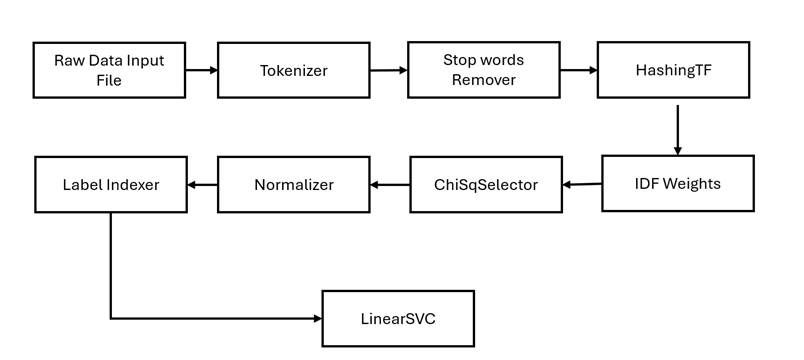
\includegraphics[width=\textwidth]{strategy.png}
  \caption{Spark-based strategy pipeline for text preprocessing and classification}
  \label{fig:pipeline-strategy}
\end{figure}


\subsection{Spark Environment Setup}

\begin{itemize}
  \item \texttt SparkSession is created with dynamic configuration depending on execution mode (local or cluster).
  \item Configuration parameters are centrally defined for dataset paths, output locations, model hyperparameters, and pipeline settings.
    \item Resources such as shuffle partitions and executor cores are dynamically tuned to match the execution environment.
\end{itemize}


\subsection{Task 1 – Chi-Square Feature Selection with RDDs}

\begin{itemize}
  \item \textbf{Data Loading:} The JSON dataset is loaded from HDFS and parsed using RDD transformations.
  \item \textbf{Preprocessing:} Text is lowercased, punctuation is removed, and a regex tokenizer is applied. Custom stopword filtering is used.
  \item \textbf{Category Pairing:} Each review is transformed into (\texttt{word}, \texttt{category}) pairs.
  \item \textbf{Chi-Square Computation:} Term frequencies and expected frequencies are used to compute chi-square values for each word.
  \item \textbf{Output Generation:} The top terms per category and a global dictionary are saved to \texttt{output\_rdd.txt}.
\end{itemize}

\subsection*{3.3 Task 2 – Spark ML Pipeline with DataFrames}

\begin{itemize}
  \item \textbf{Tokenization:} Used \texttt{RegexTokenizer} to split review text based on punctuation, digits, and whitespace.
  \item \textbf{Stopword Removal:} Applied \texttt{StopWordsRemover} to remove common uninformative words.
  \item \textbf{TF-IDF Transformation:} \texttt{HashingTF} and \texttt{IDF} are used to convert text to TF-IDF-weighted feature vectors.
  \item \textbf{Label Encoding:} Categories are indexed numerically with \texttt{StringIndexer}.
  \item \textbf{Chi-Square Selection:} Used \texttt{ChiSqSelector} to select the top 2000 terms across all classes.
  \item \textbf{Pipeline Construction:} All transformations are assembled into a \texttt{Pipeline} and executed on the dataset.
  \item \textbf{Output:} Selected terms are stored in \texttt{output\_ds.txt}.
\end{itemize}

\subsection*{3.4 Task 3 – Text Classification with SVM}

\begin{itemize}
  \item \textbf{Normalization:} Feature vectors are normalized using \texttt{Normalizer} with L2 norm.
  \item \textbf{Classification:} \texttt{LinearSVC} with \texttt{OneVsRest} is used for multi-class classification.
  \item \textbf{Data Splitting:} The data is split into training (80\%), validation (10\%), and test (10\%) sets.
  \item \textbf{Hyperparameter Tuning:} Used \texttt{ParamGridBuilder} and \texttt{TrainValidationSplit} to explore:
    \begin{itemize}
      \item Regularization parameter: \texttt{0.01}, \texttt{0.1}, \texttt{1.0}
      \item Standardization: enabled/disabled
      \item Max iterations: \texttt{50}, \texttt{100}
    \end{itemize}
  \item \textbf{Evaluation:} Used \texttt{MulticlassClassificationEvaluator} with F1-score as the metric.
\end{itemize}



\section{Code Documentation}

This section outlines the major functions, Spark components, and logical flow implemented for each task in the project.

\subsection*{Task 1 – RDD-Based Chi-Square Feature Selection}
\begin{itemize}
  \item \texttt{parse\_review(line)} – Parses each JSON review line and extracts its category and review text.
  \item \texttt{preprocess\_text(text)} – Tokenizes, lowercases, removes stopwords and short tokens.
  \item \texttt{compute\_chi(kv)} – Computes chi-square statistics for a given (category, term) pair.
  \item \texttt{topk\_per\_category(iterator)} – Aggregates top-K scoring terms per category using a local heap.
  \item \texttt{clean\_term(term)} – Cleans terms by stripping non-alphanumeric characters.
\end{itemize}

\subsection*{Task 2 – TF-IDF and Feature Selection with DataFrames}
\begin{itemize}
  \item \texttt{RegexTokenizer} – Splits text into tokens based on regular expression patterns.
  \item \texttt{StopWordsRemover} – Filters out stopwords from the tokenized text.
  \item \texttt{CountVectorizer} – Converts filtered tokens into sparse term frequency vectors.
  \item \texttt{IDF} – Applies inverse document frequency weighting to TF vectors.
  \item \texttt{StringIndexer} – Encodes category labels into indexed numeric values.
  \item \texttt{ChiSquareTest.test()} – Evaluates each feature's relevance using chi-square statistics.
\end{itemize}

\subsection*{Task 3 – Classification Pipeline and Evaluation}
\begin{itemize}
  \item \texttt{ChiSqSelector} – Selects top-N features based on chi-square relevance to the target label.
  \item \texttt{StandardScaler} – Standardizes feature vectors to improve classifier stability.
  \item \texttt{Normalizer} – Normalizes vectors using L2 norm to ensure consistent scaling.
  \item \texttt{LinearSVC} – Defines a linear support vector classifier for binary tasks.
  \item \texttt{OneVsRest} – Extends LinearSVC to multi-class classification using one-vs-rest strategy.
  \item \texttt{ParamGridBuilder} – Constructs a grid of hyperparameter combinations for model tuning.
  \item \texttt{TrainValidationSplit} – Performs model selection using train/validation splits and F1 score.
  \item \texttt{MulticlassClassificationEvaluator} – Computes F1 score for multi-class predictions.
  \item \texttt{bestModel.stages[]} – Retrieves the optimal model pipeline and its learned parameters.
\end{itemize}



\clearpage
\section{Results}

This section summarizes the runtime performance, outputs, and key findings from each task executed using Apache Spark. All experiments were run on a distributed environment using HDFS and were optimized for performance and reproducibility.

\subsection{Task 1 – RDD-Based Chi-Square Feature Selection}
\begin{itemize}
  \item \textbf{Runtime:} 30.48 seconds (includes both computation and file writing).
  \item \textbf{Output:} Top 75 chi-square terms were extracted for each product category based on token frequency and category association.
  \item \textbf{Observations:} Discriminative terms such as \texttt{games} (Apps), \texttt{shampoo} (Beauty), and \texttt{diaper} (Baby) were successfully identified, demonstrating the effectiveness of RDD-based frequency aggregation and scoring.
\end{itemize}

\subsection{Task 2 – TF-IDF and Chi-Square with DataFrames}
\begin{itemize}
  \item \textbf{Runtime:} 42.22 seconds (including output saving).
  \item \textbf{Output:} Top 2000 global features were selected using Spark ML’s \texttt{ChiSquareTest} over TF-IDF vectors.
  \item \textbf{Observations:} Results confirmed that the DataFrame pipeline is more scalable and modular. Frequently selected terms such as \texttt{iphone}, \texttt{dvd}, and \texttt{carseat} matched those in Task 1, validating consistency.
\end{itemize}

\subsection{Task 3 – Classification and Evaluation}
\begin{itemize}
  \item \textbf{Model Pipeline:} Reused TF-IDF vectors from Task 2 and added:
    \texttt{ChiSqSelector}, \texttt{StandardScaler}, \texttt{Normalizer}, and \texttt{OneVsRest(LinearSVC)}.
  \item \textbf{Tuning Parameters:}
    \begin{itemize}
      \item \texttt{regParam}: \{0.01, 0.1, 1.0\}
      \item \texttt{maxIter}: \{5, 10\}
      \item \texttt{withStd}: \{True, False\}
    \end{itemize}
  \item \textbf{Evaluation Metric:} F1 Score on the test set.
  \item \textbf{Test F1 Score:} \texttt{0.7510}
  
  \item \textbf{Best Model Parameters:}
    \begin{itemize}
      \item \texttt{numTopFeatures}: 2000
      \item \texttt{withStd}: True
      \item \texttt{regParam}: 1.0
      \item \texttt{maxIter}: 10
    \end{itemize}
\end{itemize}

\subsection{Summary}
All three tasks achieved consistent results in terms of term selection and classification performance. The TF-IDF + Chi-square feature selection aligned well with expected domain keywords, and the classification pipeline achieved a robust F1 score, confirming the pipeline’s effectiveness for multi-class review categorization.




\end{document}
